\subsection{Presensi}
Menurut Kamus Besar Bahasa Indonesia (KBBI)~\cite{kbbionline}, presensi diartikan sebagai kehadiran. Kehadiran itu sendiri mengacu pada kehadiran individu atau kelompok di suatu tempat untuk mengikuti acara yang telah direncanakan sebelumnya. Kehadiran karyawan berperan penting dalam menentukan kinerja mereka dalam menyelesaikan tugas~\cite{narulita2024buku}.

\subsection{Aplikasi Presensi}
Aplikasi adalah perangkat lunak yang dirancang untuk menjalankan tugas tertentu pada sistem komputer. Dalam pengembangannya, aplikasi dikategorikan menjadi 3 yaitu aplikasi web, aplikasi \textit{desktop}, dan aplikasi \textit{mobile}.~\cite{pane2020membangun}. Sedangkan, presensi merupakan kehadiran. Maka aplikasi presensi dapat disebut sebagai perangkat lunak yang digunakan untuk mencatat dan memantau kehadiran suatu individu. Menurut Imaniawan dan Rijanandi~\cite{imaniawan2023presensi}, aplikasi presensi memungkinkan pengelolaan data kehadiran secara efisien dikarenakan data dari presensi langsung tersimpan pada server.

\subsection{Lembur}
Menurut Kamus Besar Bahasa Indonesia (KBBI)~\cite{kbbionline}, Lembur merupakan pekerjaan dinas yang dilakukan diluar jam dinas. Berdasarkan Keputusan Menteri Tenaga Kerja Republik Indonesia Nomor KEP. 102 Men VI 2004 pasal 1~\cite{menteri2014peraturan}, perusahaan diwajibkan untuk membayar upah lembur kepada pegawai jika masuk pada kategori berikut:
\begin{enumerate}
    \item Bekerja lebih dari 7 jam dalam sehari atau 40 jam dalam seminggu untuk pegawai yang bekerja selama 6 hari.
    \item Bekerja lebih dari 8 jam sehari dan 40 jam dalam seminggu untuk pegawai yang bekerja selama 5 hari.
    \item Bekerja pada hari istirahat mingguan dan hari libur nasional.
\end{enumerate}

\subsection{\textit{Geolocation}}
Menurut Shellito~\cite{introduction2019bradley}, \textit{Geolocation} adalah teknik yang digunakan untuk menentukan lokasi suatu perangkat di dunia nyata, seperti \textit{smartphone}, tablet, atau komputer. Dengan \textit{Geolocation}, perangkat dapat mengetahui koordinatnya (lintang dan bujur) melalui berbagai metode, seperti alamat IP, koneksi Wi-Fi, menara seluler, atau GPS. Setelah lokasi ditentukan, informasi tersebut dapat dipetakan dan dibagikan melalui internet.

\subsection{Haversine}
Haversine merupakan metode paling populer yang menggunakan trigonometri untuk menghitung jarak lingkaran besar dengan menggunakan koordinat yang didefinisikan dalam derajat desimal sebagai \textit{input}. Rumus Haversine adalah rumus pengukuran jarak yang paling umum digunakan karena relatif ringan dari segi pengkodean dan cukup akurat dalam kebanyakan kasus~\cite{learning2019joel}. Menurut Xiao~\cite{gis2015xiao}, langkah pertama pada rumus Haversine yaitu mencari nilai a atau nilai antara yang dapat dilihat pada \textbf{Persamaan \ref{eq:nilai-a}}.
\begin{equation}
    a = \sin^2 \left( \frac{d\varphi}{2} \right) + \cos(\varphi_1) \cdot \cos(\varphi_2) \cdot \sin^2 \left( \frac{d\lambda}{2} \right)
\label{eq:nilai-a}
\end{equation}


\noindent Keterangan:
\\
$d\varphi$ = Perbedaan lintang antara dua titik ($\varphi_2 - \varphi_1$).
\\
$\varphi_1$ = Lintang titik pertama (dalam radian).
\\
$\varphi_2$ = Lintang titik kedua (dalam radian).
\\
$d\lambda$ = Perbedaan bujur antara dua titik ($\lambda_2 - \lambda_1$).
\\
$\lambda_1$ = Bujur titik pertama (dalam radian).
\\
$\lambda_2$ = Bujur titik kedua (dalam radian).
\\

Selanjutnya, mencari nilai c atau jarak sudut antara dua titik pada permukaan bola dalam radian menggunakan nilai a yang sudah didapatkan sebelumnya yang dapat dilihat pada \textbf{Persamaan \ref{eq:nilai-c}}.
\begin{equation}
    c = 2 \, \text{arcsin} \left( \min(1, \sqrt{a}) \right)
\label{eq:nilai-c}
\end{equation}

Setelah itu, mencari nilai d atau jarak sebenarnya antara dua titik dalam permukaan bumi dengan mengalikan nilai jarak sudut (c) dengan jari-jari bumi (6371 km) yang dapat dilihat pada \textbf{Persamaan \ref{eq:nilai-d}}.
\begin{equation}
    d = cR
\label{eq:nilai-d}
\end{equation}

Berikut ini adalah contoh perhitungan manual menggunakan rumus Haversine antara titik koordinat Universitas Tarumanagara (-6.19058187063816, 106.79779495106814) dengan titik koordinat MyPassword (-6.169336170685656, 106.78859045462738). Langkah pertama adalah melakukan konversi lintang dan bujur kedua titik menjadi radian dan mencari nilai perbedaan lintang dan bujur antara dua titik.
\\
$\varphi_1 = -6,19058187063816 \cdot \left( \frac{\pi}{180} \right) = -0.10804603626 $ radian 
\\
$\lambda_1 = 106,79779495106814 \cdot \left( \frac{\pi}{180} \right) = 1,86397315577 $ radian
\\
$\varphi_2 = -6,169336170685656 \cdot \left( \frac{\pi}{180} \right) = -0,10767522884 $ radian
\\
$\lambda_2 = 106,78859045462738 \cdot \left( \frac{\pi}{180} \right) = 1,86381250700 $ radian
\\
$d\varphi = -0,10767522884 - (-0,10804603626) = 0,00037080742 $ radian
\\
$d\lambda = 1,86381250700 - 1,86397315577 = -0,00016064877 $ radian
\\


Setelah melakukan pengubahan semua lintang dan bujur menjadi radian. Selanjutnya, melakukan perhitungan untuk mencari nilai $c$ atau jarak sudut antara dua titik.
\\
$a = \sin^2 \left( \frac{0,00037080742}{2} \right) + \cos(-0.10804603626) \cdot \cos(-0,10767522884) \cdot \sin^2 \left( \frac{-0,00016064877}{2} \right)$
\\
$a = (0,0001854037)^2 + 0,99416870319 \cdot 0,9942086212 \cdot  (-0,00008032438)^2 $
\\
$a = 3,4374535 $ x $10^-8$ + $0,99416870319 \cdot 0,9942086212 \cdot 6,452007$ x $10^-9 $
\\
$a = 4,0751770 $ x $ 10^-8 $
\\


Selanjutnya menghitung nilai c atau jarak sudut antara dua titik menggunakan nilai a atau nilai antara yang sudah didapatkan sebelumnya.
\\
$c = 2 \cdot \, \text{arcsin} \left( \min(1, \sqrt{4,0751770 \, \text{x} \, 10^-8}) \right)$
\\
$c = 2 \cdot \, \text{arcsin} \, 0,00020187066 $
\\
$c = 0,00040374135 $
\\

Terakhir, menghitung jarak dua titik dalam permukaan bumi menggunakan nilai c atau jarak sudut antara dua titik dengan jari-jari bumi (6371 km).
\\
$d = 0,00040374135 \cdot 6371 $
\\
$d = 2,5722361635632 $
\\


Jadi, hasil jarak yang dihitung antara Universitas Tarumanagara dan MyPassword menggunakan rumus Haversine adalah 2,57 km.



\subsection{\textit{World Wide Web} atau Web}
\textit{World Wide Web} (WWW) atau Web adalah sebuah aplikasi perangkat lunak yang memudahkan dan memungkinkan hampir semua orang untuk menerbitkan dan menjelajahi dokumen \textit{hypertext} pada internet~\cite{zero2022jain}. Web menggunakan protokol HTTP, yang merupakan salah satu dari sekian banyak bahasa yang digunakan di Internet untuk mengirimkan data. Web juga memanfaatkan \textit{browser} seperti \textit{Internet Explorer} atau \textit{Firefox} untuk membuka dokumen Web yang dikenal sebagai halaman Web. Halaman-halaman ini terhubung satu sama lain melalui \textit{hyperlink}. Dokumen \textit{Web} dapat berisi grafik, suara, teks, dan video~\cite{sastradipraja2022konsep}.

\subsection{\textit{Website}}
\textit{Website} adalah media dengan banyak halaman yang saling terhubung (\textit{hyperlink}) dan berfungsi untuk memberikan informasi dalam bentuk teks, gambar, video, suara, dan animasi. \textit{Website} modern umumnya bersifat dinamis, sedangkan \textit{website} statis kini jarang ditemukan. Halaman-halaman pada \textit{website} terhubung dan diakses melalui \textit{domain} (URL) di \textit{World Wide Web} (WWW), serta menggunakan \textit{hosting} untuk menyimpan data. \textit{Website} diakses menggunakan \textit{browser} seperti \textit{Chrome, Mozilla Firefox, Internet Explorer} (IE), dan \textit{Opera}~\cite{2020buku}. Menurut Asari \textit{et al}.~\cite{andipengembangan}, \textit{website} dibagi menjadi 2 yaitu \textit{web} dinamis yang merupakan \textit{web} tanpa \textit{database} dikarenakan isi \textit{web} tersebut tidak akan berubah informasinya, sedangkan \textit{web} dinamis merupakan \textit{web} yang isi halamannya selalu berubah secara berkala. Contoh \textit{website} dapat dilihat pada \textbf{\ref{fig:contoh-website}}.
%
\begin{figure}[!htbp]
	\centering
	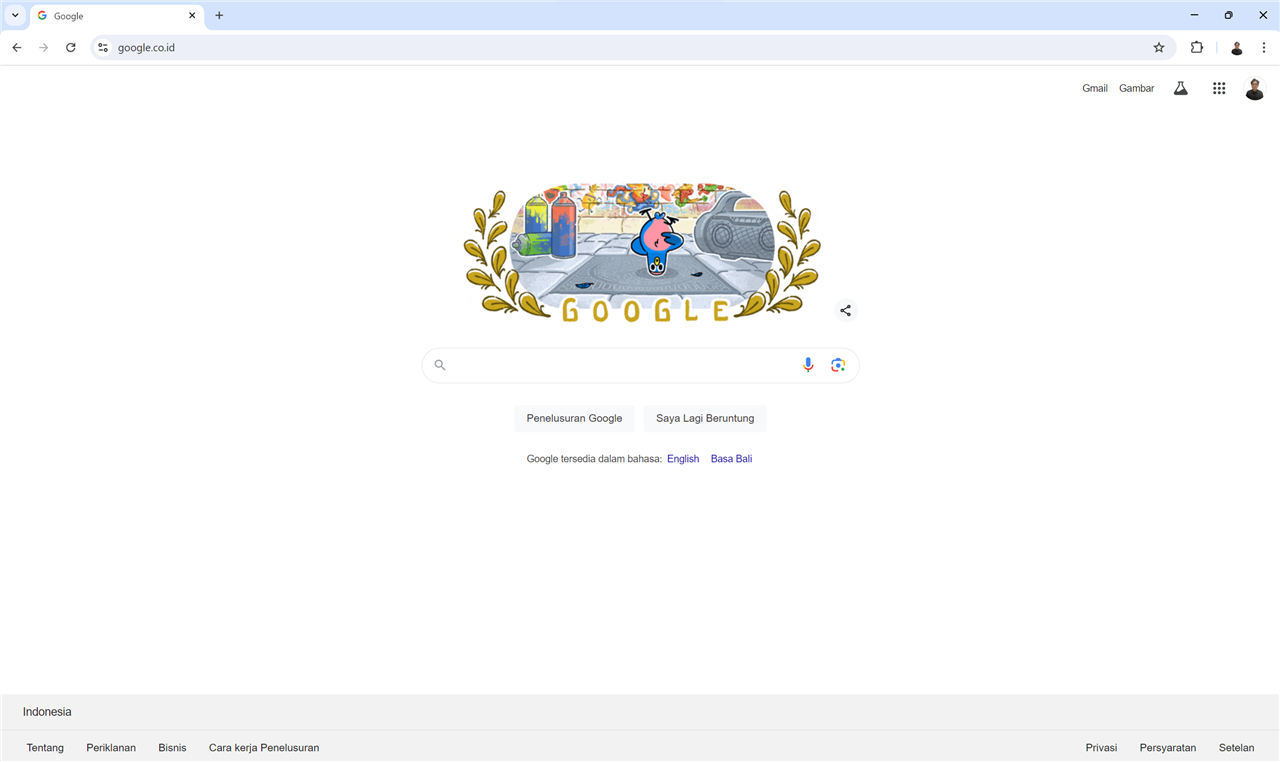
\includegraphics[width=10cm]{Gambar/bab2/website.png}
	\caption{Contoh \textit{Website}~\cite{website2024google}}
	\label{fig:contoh-website}
\end{figure}
\FloatBarrier
%
\subsection{\textit{Web Page}}
Menurut Kumar~\cite{web2018akshi}, \textit{Web page} merupakan dokumen yang ditampilkan pada \textit{web browser}. \textit{Web page} bisa bersifat statis atau dinamis. Statis berarti halaman tersebut tetap sama atau tidak berubah, sementara dinamis berarti halaman tersebut dapat berubah. Oleh karena itu, halaman web statis berisi konten yang sama setiap kali halaman dimuat, sedangkan konten halaman web dinamis dapat dihasilkan secara langsung saat dibutuhkan. Pada \textbf{\ref{fig:contoh-web-page}} merupakan contoh \textit{web page} dengan url \url{https://www.microsoft.com/id-id/microsoft-365} yang merupakan bagian satu halaman dari \textit{website} \url{https://www.microsoft.com/id-id/}.
%
\begin{figure}[!htbp]
	\centering
	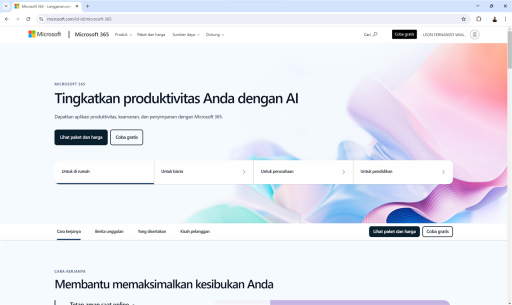
\includegraphics[width=10cm]{Gambar/bab2/web-page.png}
	\caption{Contoh \textit{Web Page}~\cite{webpage2024microsoft}}
	\label{fig:contoh-web-page}
\end{figure}
\FloatBarrier
%

\subsection{\textit{Scrum}}
Scrum adalah kerangka kerja yang dirancang untuk menerapkan prinsip-prinsip Agile dalam pengembangan. Konsep Scrum pertama kali diperkenalkan dalam artikel berjudul "The New New Product Development Game" oleh Takeuchi dan Nonaka, yang diterbitkan oleh Harvard Business Review (HBR) pada tahun 1986~\cite{magdalena2023scrum}. Menurut Hooda dkk.~\cite{hooda2023agile}, \textit{Scrum} terdiri dari 3 tahap utama yaitu \textit{outline planning}, \textit{sprint cycle}, dan \textit{project closure} yang dapat dilihat pada \textbf{\ref{fig:scrum-phases}}.
\begin{enumerate}
    \item \textit{Outline Planning}
    \\
    Pada tahap pertama, penulis akan melakukan analisis dan identifikasi kebutuhan pengguna untuk perangkat lunak. Pada tahap ini, \textit{product backlog} juga disusun, berisi daftar fitur yang dibutuhkan oleh perangkat lunak, yang diurutkan berdasarkan prioritas.
    
    \item \textit{Sprint Cycle}
    \\
    Pada tahap ini, \textit{sprint} dimulai dengan \textit{sprint planning}, yaitu proses pemilihan item dari \textit{product backlog} yang akan dikerjakan dalam setiap \textit{sprint}. Setiap \textit{sprint} berlangsung dalam iterasi pendek yang biasanya berkisar antara 1 hingga 4 minggu. Pada iterasi ini akan berfokus pada penyelesaian \textit{item} yang telah dipilih. Pada akhir setiap \textit{sprint} akan dilakukan \textit{sprint review} untuk memastikan bahwa item yang dikerjakan sudah sesuai memenuhi kriteria yang diharapkan. Siklus sprint ini akan terus berulang sampai semua item pada \textit{product backlog} terselesaikan atau proyek sudah mencapai tujuannya.

    \item \textit{Project Closure}
    \\
    Tahap terakhir adalah fase penutupan, di mana proyek diselesaikan dan ditutup secara resmi. Aktivitas yang dilakukan di tahap ini mencakup penyelesaian dokumentasi yang diperlukan, seperti panduan sistem atau manual pengguna.
\end{enumerate}
%
\begin{figure}[!htbp]
	\centering
	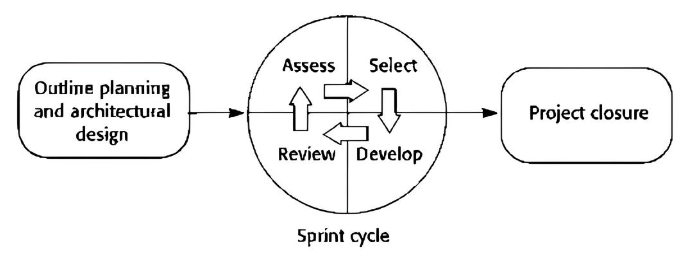
\includegraphics[width=10cm]{Gambar/bab2/scrum-methodology.png}
	\caption{\textit{Scrum Phases}~\cite{sommerville2014software}}
	\label{fig:scrum-phases}
\end{figure}
\FloatBarrier
%
Menurut Pagotto~\cite{7521555}, Metode \textit{scrum} dapat dilakukan secara individu atau sendiri yang disebut sebagai \textit{scrum solo}. \textit{Scrum Solo} memiliki karakteristik mirip dengan \textit{scrum}, seperti \textit{backlog} produk dan \textit{sprint}. Namun, \textit{scrum Solo} menggunakan \textit{sprint} satu minggu tanpa pertemuan harian. Di akhir setiap \textit{sprint}, pengembang harus menyampaikan prototipe perangkat lunak baru, dan pertemuan dengan klien atau pengguna akhir dilakukan jika diperlukan. \textit{Scrum Solo} mengintegrasikan praktik baik dari \textit{scrum} dengan fleksibilitas tambahan. Berikut ini adalah beberapa aktor proses untuk pengembangan secara individu:
\begin{enumerate}
    \item \textit{Product Owner}
    \\
    Pemilik produk yang bertanggung jawab atas visi dan arah dari produk, berinteraksi langsung dengan produk, baik sebagai individu atau sekelompok pengguna serta memastikan bahwa produk memenuhi kebutuhan pengguna dan tujuan bisnis. Mereka memberikan arahan dan keputusan penting tentang fitur dan prioritas produk.

    \item \textit{Individual Developer}
    \\
    Pengembang individu yang bertanggung jawab untuk menjalankan proses pengembangan dan membangun produk. Memiliki peran menulis kode, mengimplementasikan fitur, memperbaiki bug, dan memastikan bahwa produk berfungsi dengan baik. \textit{Individual Developer} memiliki tanggung jawab mengikuti spesifikasi dan arahan yang diberikan oleh \textit{Product Owner}, dan memastikan bahwa produk dikembangkan sesuai dengan standar dan tenggat waktu yang ditetapkan.

    \item \textit{Advisor}
    \\
     Konsultan yang memiliki pengetahuan mendalam tentang proses pengembangan. \textit{Advisor} memiliki peran Memberikan saran dan panduan tentang teknologi yang digunakan dan cakupan proyek dan bertanggung jawab menyediakan wawasan luas tentang teknologi dan metodologi yang digunakan dalam pengembangan produk, serta membantu tim dalam mengatasi tantangan teknis dan strategis.

     \item \textit{Validation Group}
     \\
     Pengguna potensial dari produk yang dihasilkan. \textit{Validation Group} memiliki peran berpartisipasi dalam proses validasi produk, dan tanggung jawab menguji produk dan memberikan umpan balik untuk memastikan bahwa produk memenuhi kebutuhan dan ekspektasi pengguna. Partisipasi mereka harus didokumentasikan dalam laporan proses.
    
\end{enumerate}

\subsection{PT Password Solusi Sistem}
Berdasarkan \textit{web} resmi MyPassword~\cite{aboutuswebsite}, MyPassword didirikan pada tahun 2009 sebagai perusahaan solusi teknologi informasi dan integrator sistem, yang menyediakan solusi infrastruktur teknologi informasi dan aplikasi bisnis, termasuk memberikan implementasi, pemeliharaan, dan layanan lainnya. Perusahaan ini dipimpin oleh dua direktur yaitu Bapak Hendriyanto Suhandi dan Bapak Julius Wendra Lea. Logo MyPassword dapat dilihat pada \textbf{\ref{fig:logo-mypassword}}.
%
\begin{figure}[!htbp]
	\centering
	
\includegraphics[width=10cm]{Gambar/bab2/logo-mypassword.png}
	\caption{Logo MyPassword~\cite{aboutuswebsite}}
	\label{fig:logo-mypassword}
\end{figure}
\FloatBarrier
%
Kantor MyPassword berlokasi di Wisma 77 \textit{Tower} 1, Lantai 15 yang dapat dilihat pada \textbf{\ref{fig:gedung-wisma-77}}, dengan alamat di Jl. Letjen S. Parman No.Kav. 77, RT.6/RW.3, Slipi, Kecamatan Palmerah, Kota Jakarta Barat, Daerah Khusus Ibukota Jakarta, 11410. MyPassword menyediakan beberapa solusi dan layanan yang ditawarkan diantaranya \textit{Modern Data Center, Modern Information System, Modern Office}, dan \textit{Modern Services}.
%
\begin{figure}[!htbp]
	\centering
	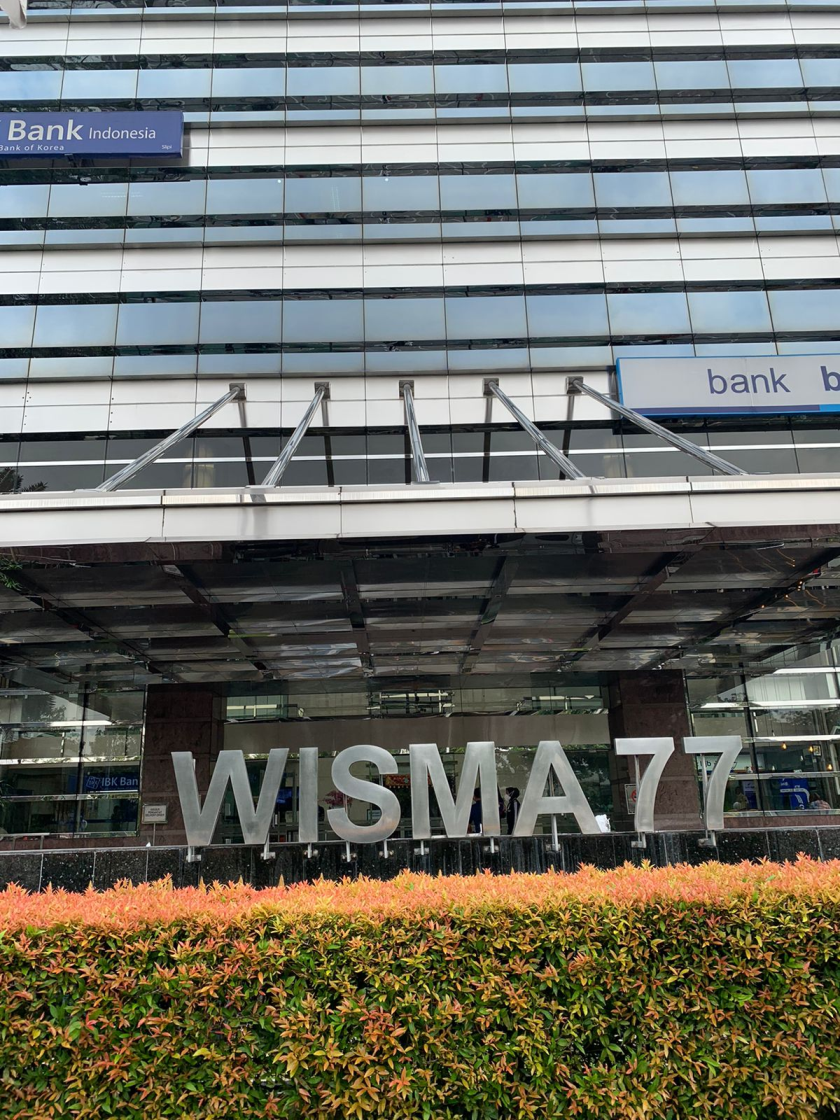
\includegraphics[width=5cm]{Gambar/bab2/gedung-wisma-77.jpeg}
	\caption{Gedung Wisma 77 \textit{Tower} 1}
	\label{fig:gedung-wisma-77}
\end{figure}
\FloatBarrier
%
MyPassword terdiri dari beberapa divisi diantaranya yaitu \textit{Business Application, Human Resources, Infrastructure, Business Support,} dan lain-lain. Jam kerja utama di kantor MyPassword yaitu Senin sampai Jumat, mulai pukul 8 pagi hingga 5 sore. Namun, untuk divisi \textit{Infrastructure} tidak semua \textit{staff} menggunakan jam kerja utama, tetapi \textit{staff Infrastructure} bekerja menggunakan jam \textit{shift} yang sudah ditentukan sehingga jam kerja mungkin akan berbeda antara satu \textit{staff} dengan \textit{staff} lainnya. Selanjutnya pada kantor MyPassword terdapat kerja lembur salah satunya divisi \textit{Infrastructure}, yang bekerja diluar jam \textit{shift} yang telah ditentukan atau bekerja pada hari libur nasional. Kerja lembur pada MyPassword juga tidak hanya dilakukan di kantor saja, tetapi juga bisa dilaksanakan di luar kantor.

Saat ini pencatatan lembur pada MyPassword sudah menggunakan aplikasi bernama "Andal". Aplikasi ini dibeli melalui pihak eksternal dengan \textit{one time payment}. Aplikasi ini dapat di-\textit{download} melalui \textit{playstore} ataupun \textit{appstore}. Pada proses bisnis aplikasi ini, \textit{Staff Infrastructure} harus melakukan presensi terlebih dahulu sebelum melakukan pengajuan lembur. Saat presensi akan dilakukan pengambilan lokasi dan foto \textit{Staff Infrastructure}. Setelah melakukan presensi maka \textit{Staff Infrastructure} dapat mengajukan formulir lembur yang mengacu pada presensi yang telah dilakukan. Jika \textit{Staff Infrastructure} lupa melakukan presensi pada hari kerja lembur maka tidak bisa melakukan pengajuan lembur sehingga \textit{Staff Infrastructure} perlu mengajukan \textit{form attendance correction} pada aplikasi. Permasalahan utama dari aplikasi yang saat ini digunakan adalah kurangnya fleksibilitas dalam penyesuaian, karena fitur-fiturnya sudah ditentukan berdasarkan layanan dari pihak ketiga. Akibatnya, ketika \textit{Staff Infrastructure} melakukan lembur lebih dari satu kali dalam sehari dalam aplikasi, perhitungan lembur harus dilakukan secara manual, yang mengakibatkan proses menjadi tidak efisien.






